\section{پیاده سازی}
برای پیاده سازی این تمرین، شما امکان استفاده از دو زبان c++ و java را دارید. پیشنهاد ما استفاده از زبان java است، چرا که مشکلات کار با اشاره‌گر‌ها را نخواهید داشت. همچنین کمتر درگیر Endianess خواهید شد و تجربه ترم‌های پیش نشان داده کار با جاوا به مراتب راحت تر است. اما از طرفی برنامه نویسی c++ بسیار جزئی‌تر است و شما کار با کتابخانه‌های اصلی و رایج را یاد می‌گیرید که به مراتب جذاب‌تر از جاوا است.

\notice{
همه‌ی برنامه‌های شما در سامانه‌عامل لینوکس با هسته‌ی ۳٫۱۹ به بالا کامپایل می‌شوند و شما هم باید کد خود را در سامانه‌عامل لینوکسی کامپایل نمایید.
}


\notice{
 در تمام این تمرین، برای شبیه‌سازی شبکه و ارسال پیام بین گره‌ها، شما نیاز به استفاده از سامانه‌ی پرتو دارید.
 }
\subsection{مشترک}
\begin{itemize}
\item
برای کار با سیستم پرتو، نام کاربری و رمز خود را در پرونده 
\code{info.sh}
 قرار دهید.
\item
برای کامپایل شدن کد خود، از دستور
\code{make}
استفاده کنید. دقت کنید که کد ارسالی شما \textbf{باید} از این طریق کامپایل شود وگرنه شما نمره‌ای نخواهید گرفت.
\item
پس از کامپایل، ابتدا به اینترنت متصل شوید. سپس جهت اجرا شدن کد، باید فایل
\code{free.sh}
را اجرا کنید تا اطلاعات نقشه قبلی از پرتو شما حذف شود. سپس، با اجرای
\code{new.sh}
یک نقشه جدید ایجاد کنید. پس از این می‌توانید کد کامپایل شده خود را با اجرای
\code{run.sh ٓ$X$}
اجرا کنید. که $X$ شماره گره‌ای از شبکه است که کد شما قرار است جای آن بنشینید.
\end{itemize}

\subsection{برنامه نویسی java}

\begin{itemize}
\item
در صورتی که زبان java را برای پیاده سازی انتخاب کردید، پیشنهاد ما استفاده از IDE Eclipse یا intelij است، تا کارتان راحت‌تر شود. شما تنها حق تغییر فایل های پکیج ir.sharif.ce.partov.machine را دارید و فایل‌های دیگر خود را نیز تنها در این بخش قرار دهید.
\item
دو فایل 
\code{ServerMachine.java}
و
\code{ClientMachine.java}
به صورت پیش فرض پر شده‌اند. شما باید این دو فایل را برای هر یک از حالت‌هایی که گره شما در نقش کارگزار DHCP و کارخواه باشد، پر کنید و منطق خود را پیاده سازی کنید.

\end{itemize}
\subsection{برنامه نویسی c++}
در صورتی که زبان c++ را انتخاب کردید، پیشنهاد ما استفاده از یکی از IDE های رایج مانند ( eclipse، intelij، codeblocks و غیره) است، چرا که ممکن است نیاز به استفاده از کتابخانه‌هایی داشته باشید که تا به حال به آن‌ها برنخورده‌اید. با امکانات این نرم‌افزار‌ها می‌توانید کار خود را راحت‌تر انجام دهید و کتابخانه‌های جدید را راحت مطالعه کنید. \\

شما باید کد اصلی خود را در دو فایل
\code{server\_machine.cpp}
و
\code{client\_machine.cpp}
قرار دهید تا هرگاه کد شما به عنوان یکی از این اعضاء اجرا شد، منطق گفته شده به درستی کار کند. \\

در صورتی‌ که می‌خواهید چند فایل دیگر نیز اضافه کنید، آن‌ها را در پوشه user قرار دهید و مطمن شوید که کد شما با روش گفته شده کامپایل می‌شود.
\subsection{نقشه نمونه}
برای راحتی کار شما، نقشه ساده‌ای جهت تست برنامه‌یتان وجود دارد با نام
\code{DHCP\_Simple}
که به شکل زیر است. دقت کنید که نقشه مورد آزمون در داوری نمرات با این نقشه متفاوت خواهد بود. \begin{figure}[h!]
	\begin{center}
 		\caption{نقشه‌ی نمونه}
		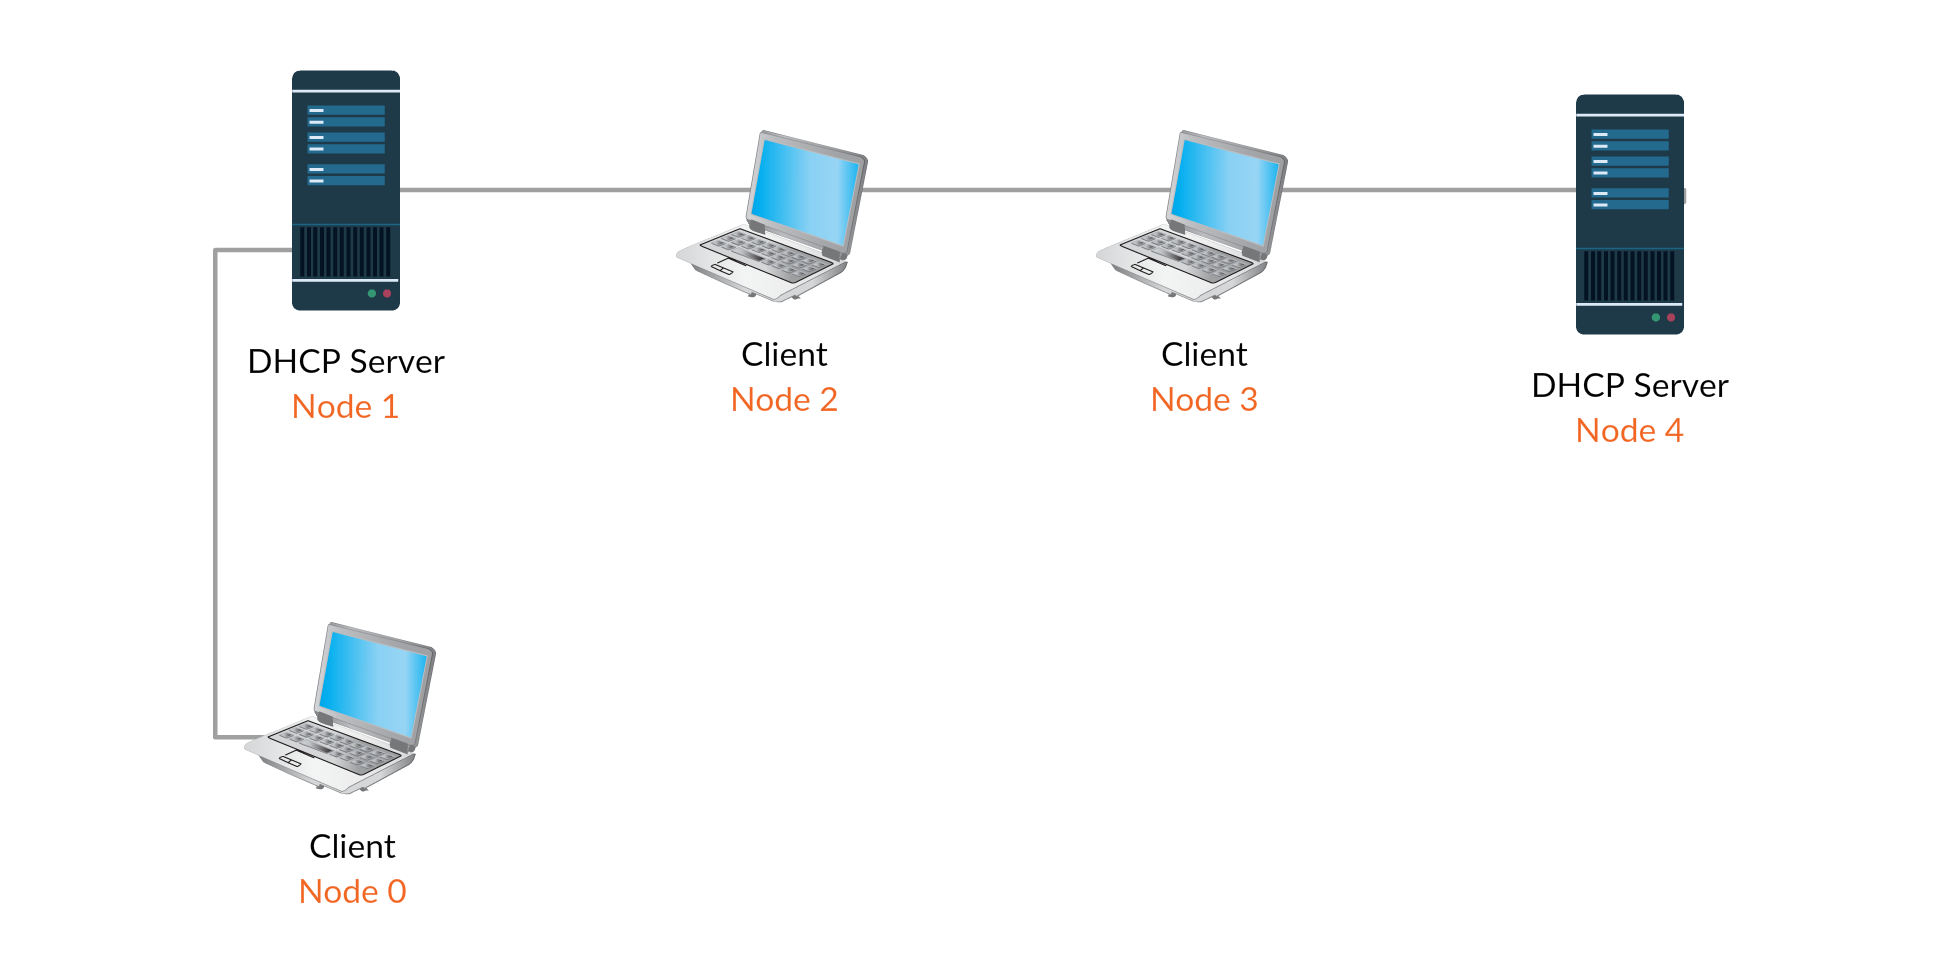
\includegraphics[scale=.4]{DHCP_Simple.png}
	\end{center}
\end{figure}
